\section{Training Examples}
\label{sec:training_examples}

Figure~\ref{fig:training_examples} shows six training examples from various sources.


\begin{figure}[b]
    \centering
    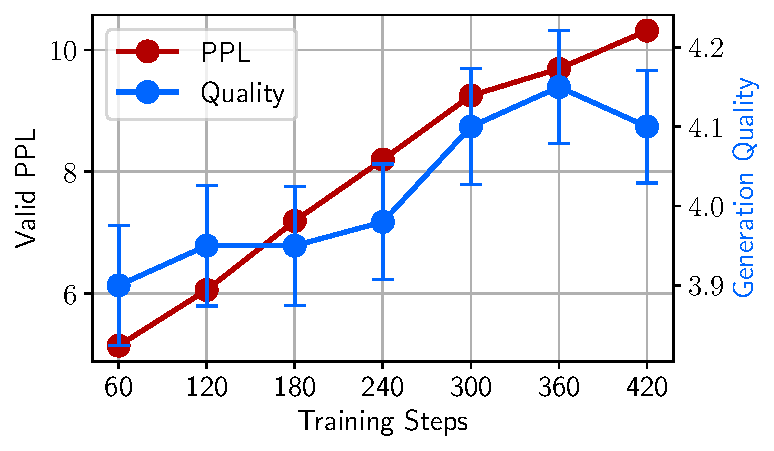
\includegraphics[width=0.5\linewidth]{figs/ppl_65b.pdf}
    \caption{Validation set perplexity versus generation quality (as evaluated by ChatGPT), across the training process of LIMA 65B. We observe similar trends for 7B and 30B parameter models, and across different mixtures of training data.}
    \label{fig:ppl}
\end{figure}



\begin{figure*}[p]
    \scriptsize
    \centering
    \begin{tabular}{@{}p{0.31\columnwidth}p{0.31\columnwidth}p{0.31\columnwidth}@{}}
    \toprule
    \textbf{[Stack Exchange (STEM)]}
    
    \textcolor[HTML]{3078BE}{\textbf{What is the difference between minimum and infimum? I have a great confusion about this.}}
    
    ~
    
    The minimum is attained, the infimum isn't necessarily. 

    ~
    
    Example: Let $f(x) = \frac{1}{x}$. Then $f$ has no minimum value on the interval $(0,\infty)$. The minimum is the smallest element in the set. That is $\min\{f(x)\mid x\in (0,\infty)\}$ doesn't exist because there is not smallest number in the set. Another example is the minimum of the set $S = (0,1) = \{x\mid 0<x<1\}$. Here again there isn't a smallest number $\min\{x\mid 0<x<1\}$ doesn't exist.

    ~
    
    The infimum of a set $S$ is defined as the greatest number that is less than or equal to all elements of S (from Wikipedia). The infimum is also sometimes called the greatest lower bound.
    It is a fact that every non empty set (bounded below) of real numbers has an infimum. But, as we saw, not every real set has a minimum.
    So in the example $\inf\{f(x)\mid x\in (0,\infty)\} = 0.$

    ~
    
    Note that the infimum and the minimum can be the same. Consider for example $S = \{1,2,3,\dots\}$. Then the infimum and minimum is both $1$.
    Consider this other example. If $f$ is a continuous function on a closed interval $[a,b]$,  then it is a fact that $f$ attains a minimum over that interval. So here again $\inf\{f(x)\mid x\in [a,b]\} = \min\{f(x)\mid x\in [a,b]\}$.
    
    &
    \textbf{[Stack Exchange (Other)]}
    
    \textcolor[HTML]{3078BE}{\textbf{Was the Millennium Falcon a one-off or was it mass produced?}}
    
    ~
    
    The Millennium Falcon is not unique; it was a model YT-1300f Corellian light freighter. This implies that there are other similar ships, including other variations on the YT-1300 model. You can find a lot of information about the Millennium Falcon in a companion book, Star Wars: The Force Awakens: Incredible Cross-Sections. The model number also appears on-screen at least once: in Star Wars: Rebels episode ``Fighter Flight'' on a poster. Note, however, that the Millennium Falcon has been highly customized; some of the custom work is mentioned in The Force Awakens. It's not clear just how much of the ship is stock and how much is custom.

    ~
    
    If you're willing to go outside Canon into Legends, the model number of the ship, and other similar Corellian light freighters, can be seen in some of the video games, and there is an entire novel called Millennium Falcon that details its history. The ship was serial \#YT-1300 492727ZED, one of many such vessels, but from the beginning the ship was shown to have some ``quirks'' to distinguish it from its counterparts. In Legends, the ship was also destroyed and rebuilt from scratch at least once, so it's arguable as to whether it's still the same ship or not.
    
    &
    \textbf{[wikiHow]}
    
    \textcolor[HTML]{3078BE}{\textbf{How to be a lazy college student?}}

    ~

    In college, unlike in high school, you are expected to take responsibility for your own learning.  It is ultimately up to you to determine how much time and effort you want to put into your schoolwork. Experts suggest that college students today work considerably fewer hours than their counterparts did in 1961.  But there is also evidence that working more hours is not necessarily the best way to be productive. A little laziness may even be good for us.

    ~
    
    \textbf{Part 1 of 3: prioritize what's important}
    \begin{enumerate}[leftmargin=8pt]
        \item Ask yourself what you want from college. There are many reasons why a college degree is desirable, not least that it is still considered highly valuable by many employers. Your own reasons for pursuing a college degree may be more personal, but spend some time working out exactly what these reasons are. Consider why college is important to you. Do you want to learn important skills like critical thinking and problem-solving? Do you want to make friends, network and get to know other people? Do you want to get good grades for further study? Do you want to get a particular job that requires a college degree? Spend some time reflecting on these questions and come up with your own answers. It might even be a good idea to write them down. This will help you to recognize what's important to you so that you can focus on the essential things.
        \item Select your major and your classes carefully. \textcolor[HTML]{808080}{[...]}
    \end{enumerate}

    \\
    \midrule
    \textbf{[Manually Authored -- Chitchat]}
    
    \textcolor[HTML]{3078BE}{\textbf{Tell me an interesting fact about geography.}}

    ~
    
    Here are some interesting facts about geography:
    \begin{itemize}[leftmargin=8pt]
        \item Bhutan is one of the most intriguing places in the world. The Buddhist kingdom is the only carbon-negative country on Earth, with strict environmental laws and cultural norms that preserve its stunning natural landscape. For similar reasons, Bhutan was one of the last countries to introduce television in 1999, and has no traffic lights to this day.
        \item There are currently few territories on Earth that are unclaimed by any sovereign state (terra nullius). One example is Bir Tawil, along the border between Egypt and Sudan, which was created by a discrepancy between borders drawn in 1899 and 1902. The territory remains unclaimed by either country, because it would entail forfeiting the much larger Halaib Triangle, which is claimed by both countries. Bir Tawil has no settled population, but the land is used by Bedouins who roam the area.
        \item The antipode of any spot on Earth \textcolor[HTML]{808080}{[...]}
    \end{itemize} 
    &
    \textbf{[Manually Authored -- Advice]}
    
    \textcolor[HTML]{3078BE}{\textbf{I'm going to NeurIPS for the first time to present the first paper I've ever published. I'm afraid I'll be alone and overwhelmed by everyone. What should I do?}}
    
    ~
    
    Going to an academic conference for the first time may seem like a bewildering experience, but if done right, conferences are a wonderful opportunity to brainstorm with experts from around the world, present your work and get feedback, and make new friends. Here are some tips for improving your conference experience:
    \begin{itemize}[leftmargin=8pt]
    \item Reach out in advance to people who have inspired your work. \textcolor[HTML]{808080}{[...]}
    \item Show curiosity about other people's work. \textcolor[HTML]{808080}{[...]}
    \item Sign up for student volunteer \textcolor[HTML]{808080}{[...]}
    \item Ask your advisor to introduce you \textcolor[HTML]{808080}{[...]}
    \item At the same time, try to socialize outside of your lab \textcolor[HTML]{808080}{[...]}
    \end{itemize}
    
    Ultimately, it is important to remember that every first-conference attendee is probably feeling a bit shy too, and that taking the first step in starting a conversation will almost always be met with a big smile! 

    &
    \textbf{[Manually Authored -- Writing]}
    
    \textcolor[HTML]{3078BE}{\textbf{I am planning to start a book club with some friends. Can you write an email invitation for the same?}}

    ~
    
    Here is an example email invitation for a book club:

    ~

    Subject: Join me for a book club!

    ~
    
    Hi [Friend's Name], how are you?

    ~
    
    I'm starting a book club with some friends, and I'd love to have you join us!

    ~
    
    The book club is a casual and fun way to read and discuss books that we love or want to learn more about, and also make new friends. We plan to meet more-or-less once a month.

    ~
    
    We're thinking of having our first meeting on [Date \& Time]. Could that work for you?

    ~
    
    Would love to see you there!

    ~
    
    Thanks,
    
    [Your Name]
    \\
    \bottomrule
    \end{tabular}
    \caption{\textbf{Training examples from different sources.} \textit{Top row:} examples mined from community Q\&A. \textit{Bottom row:} manually-authored examples. The \textcolor[HTML]{3078BE}{blue} text is the prompt. The gray ellipsis \textcolor[HTML]{808080}{[...]} indicates that the response was trimmed to fit this page, but the actual training example is longer.}
    \label{fig:training_examples}
\end{figure*}



\section{Anticorrelation between Perplexity and Generation Quality}
\label{sec:ppl}

When fine-tuning LIMA, we observe that perplexity on held-out Stack Exchange data (2,000 examples) negatively correlates with the model's ability to produce quality responses.
To quantify this manual observation, we evaluate model generations using ChatGPT, following the methodology described in Section~\ref{sec:ablations}.
Figure~\ref{fig:ppl} shows that as perplexity rises with more training steps -- which is typically a negative sign that the model is overfitting -- so does the quality of generations increase.
Lacking an intrinsic evaluation method, we thus resort to manual checkpoint selection using a small 50-example validation set.



\section{Human Annotation}
\label{sec:annotation}

Figure~\ref{fig:human_annot} shows the human annotation interface we used to collect preference judgments. Annotators were asked to exercise empathy and imagine that they were the original prompters.

 \begin{figure*}[p]
    \scriptsize
    \centering
    \begin{tabular}{@{}p{0.475\columnwidth}p{0.475\columnwidth}@{}}
    \toprule

    \multicolumn{2}{@{}p{\columnwidth}@{}}{
    % \textbf{Task Description:}
    % 
    \textcolor[HTML]{3078BE}{\textbf{Imagine that you have a super-intelligent AI assistant, and that you require help with the following question. Which answer best satisfies your needs?}}
    
    ~
    
    }
    \\
    % \midrule
    
    \multicolumn{2}{@{}p{\columnwidth}@{}}{\textbf{Question:}~~<QUESTION> 

    ~

    }
    \\
    
    % \midrule
    \textbf{Answer A:}
    
    ~
    
    <ANSWER A>
    & 

    \textbf{Answer B:}
    
    ~
    
    <ANSWER B>\\
    \multicolumn{2}{@{}p{\columnwidth}@{}}{

    ~
    
    }\\
    % \midrule
    \textbf{Comparing these two answers, which answer is better?}
    \begin{itemize}[leftmargin=18pt]
       \item[$\mdblksquare$] Answer A is significantly better.
       \item[$\mdblksquare$] Answer B is significantly better.
       \item[$\mdblksquare$] Neither is significantly better.
    \end{itemize}\\
    \bottomrule
    \end{tabular}
    \caption{Human annotation interface.}
    \label{fig:human_annot}
\end{figure*}



\section{ChatGPT Score}
\label{sec:gpt_annotation}

Automatically evaluating generative models is a difficult problem.
For ablation experiments (Section~\ref{sec:ablations}), we use ChatGPT (GPT-3.5 Turbo) to evaluate model outputs on a 6-point Likert score given the prompt in Figure~\ref{fig:eval_prompt_single}.


\begin{figure}[t]
    \scriptsize
    % \texttt
    \centering
\begin{tabular}{@{}p{\columnwidth}@{}}
\toprule
You are evaluating a response that has been submitted for a particular task, using a specific set of standards. Below is the data:

~

[BEGIN DATA]

***

[Task]: \{task\}

***

[Submission]: \{submission\}

***

[Criterion]: helpfulness:

"1": "Not helpful - The generated text is completely irrelevant, unclear, or incomplete. It does not provide any useful information to the user."

"2": "Somewhat helpful - The generated text has some relevance to the user's question, but it may be unclear or incomplete. It provides only partial information, or the information provided may not be useful for the user's needs."

"3": "Moderately helpful - The generated text is relevant to the user's question, and it provides a clear and complete answer. However, it may lack detail or explanation that would be helpful for the user."

"4": "Helpful - The generated text is quite relevant to the user's question, and it provides a clear, complete, and detailed answer. It offers additional information or explanations that are useful for the user. However, some of the points of the response are somewhat repetitive or could be combined for greater clarity and concision"

"5": "Very helpful - The generated text is highly relevant to the user's question, and it provides a clear, complete, and detailed answer. It offers additional information, explanations, or analogies that are not only useful but also insightful and valuable to the user. However, the structured of the response is not well-organized and there is no clear progression or logical sequence of different points in the response."

"6": "Highly helpful -  The generated text provides a clear, complete, and detailed answer. It offers additional information or explanations that are not only useful but also insightful and valuable to the user. The response is also in a logical and easy-to-follow manner by explicitly using headings, bullet points, or numbered lists to break up the information and make it easier to read."

***

[END DATA]

~

Does the submission meet the criterion? First, write out in a step by step manner your reasoning about the criterion to be sure that your conclusion is correct. Avoid simply stating the correct answers at the outset. Then print the choice only from ``1, 2, 3, 4, 5, 6'' (without quotes or punctuation) on its own line corresponding to the correct answer. At the end, repeat just the selected choice again by itself on a new line.\\
\bottomrule
\end{tabular}
    \caption{Prompt for ChatGPT evaluation with a 6-scale Likert score. The placeholders "{task}" and "{submission}" will be replaced by specific details from the actual case being evaluated.}
    \label{fig:eval_prompt_single}
\end{figure}


% \begin{figure}[t]
%     \centering
% \begin{lstlisting}
% You are evaluating two responses that has been submitted for a particular task, using a specific set of standards. Below is the data:
% [BEGIN DATA]
% ***
% [Task]: {input}
% ***
% [Submission1]: {Submission1}

% [Submission2]: {Submission2}
% ***
% [Criterion]: helpfulness: "Helpfulness: Does the answer directly solve the question?"
% ***
% [END DATA]
% Comparing these two submissions, which one is better? First, write out in a step by step manner your reasoning about the criterion to be sure that your conclusion is correct. Avoid simply stating the correct answers at the outset. Choose one of the following options:
% A: Submission1 is significantly better.
% B: Submission2 is significantly better.
% C: Neither is significantly better.

% Directly type in "A" or "B" or "C" (without quotes or punctuation) on its own line corresponding to the correct answer. At the end, repeat just the letter again by itself on a new line.
% Reasoning:
% \end{lstlisting}
%     \caption{Prompt for system pair evaluation, where ``\{task\}'', ``\{submission1\}'' and ``\{submission2\}'' will be instantiated by an actual case.
%     }
%     \label{fig:eval_prompt_pair}
% \end{figure}



\section{Generating Text with Complex Structure}
\label{sec:structure}

In our preliminary experiments, we find that although LIMA can respond to many questions in our development set well, it cannot consistently respond to questions that specify the structures of the answer well, e.g. summarizing an article into bullet points or writing an article consisting of several key elements. 
Hence, we investigate whether adding a few training examples in this vein can help LIMA generalize to prompts with unseen structural requirements.
We added six examples with various formatting constraints, such as generating a product page that includes \textit{Highlights}, \textit{About the Product}, and \textit{How to Use} or generating question-answer pairs based on a given article.

After training with these six additional examples, we test the model on a few questions with format constraints and observe that LIMA responses greatly improve.
We present two examples in Figure~\ref{fig:structure_examples}, from which we can see that LIMA fails to generate proper answers without structure-oriented training examples (left column), but it can generate remarkably complex responses such as a marketing plan even though we do not have any marketing plan examples in our data (right column).

 \begin{figure*}[p]
    \scriptsize
    \centering
    \begin{tabular}{@{}p{0.475\columnwidth}p{0.475\columnwidth}@{}}
    \toprule
    \textbf{LIMA w/o 6 Format Constraint Examples (994 Examples)} &  \textbf{LIMA (1,000 Examples)}\\
    \midrule
    \multicolumn{2}{@{}p{\columnwidth}@{}}{
    \textbf{[Marketing Plan (Out of Distribution)]}
    
    \textcolor[HTML]{3078BE}{\textbf{I want to start a local coffee shop. Create a marketing plan with the following elements: Marketing Goals and Objectives, Define Target Audience, Research Marketing Tactics, Plan Marketing Tactics and Develop Your Timeline and Budget.}}}\\
    \midrule
    Coffee Shop Marketing Plan
    
    ~
    
    Executive Summary

    ~
    The following marketing plan for Java Jolt Coffee Bar outlines an aggressive approach to establishing a thriving coffee shop business in downtown Pittsburgh. Java Jolt will capitalize on the popularity of specialty coffees and the growing demand for WiFi hot spots by offering a comfortable environment where customers can enjoy premium coffee drinks while taking advantage of free Internet access.
    
    ~
    Market research indicates that there is a significant opportunity for a new coffee bar located in the heart of the downtown business district. Market trends suggest that consumers are willing to pay a higher price for quality specialty coffees served in a welcoming atmosphere. Additionally, many office workers and students living in the area do not have easy access to high-speed Internet service, presenting an additional revenue stream for the coffee bar.

    ~
    
    This marketing plan includes the following elements:
    \begin{itemize}[leftmargin=8pt]
    \item Market Research supporting the need for a new coffee shop in the target location
    \item Detailed Description of the products and services offered by Java Jolt
    \item Target Market Analysis identifying the primary customer segments for Java Jolt
    \item Marketing Strategy including pricing decisions, promotional activities, and ways to differentiate Java Jolt from competitors
    \item Implementation Plan detailing the actions necessary to launch Java Jolt successfully
    \item Budget allocating funds to each component of the marketing plan
    \end{itemize}

    ~

    A comprehensive marketing plan has been developed based on extensive research into the local market conditions, consumer trends, and competitive landscape. With its unique combination of premium coffee drinks and wireless Internet access, Java Jolt will quickly become a favorite destination for people seeking a relaxing environment to socialize, study, or conduct business.
    
    &    
    Here's a marketing plan for your local coffee shop.
    ~
    
    \textbf{Marketing Goals and Objectives}
    \begin{itemize}[leftmargin=8pt]
        \item Increase awareness of our brand among consumers \textcolor[HTML]{808080}{[...]}
        \item Drive foot traffic \textcolor[HTML]{808080}{[...]} during slow business hours \textcolor[HTML]{808080}{[...]}
        \item Build relationships with influencers in our community who \textcolor[HTML]{808080}{[...]}
    \end{itemize}
    
    \textbf{Define Target Audience}
    ~
    
    Our target audiences include:
    \begin{itemize}[leftmargin=8pt]
        \item Residents of the neighborhood surrounding our coffee shop
        \item Office workers near our coffee shop
        \item Students at nearby schools
    \end{itemize}
We will focus our marketing efforts on these audiences because they are most likely to become regular customers at our \textcolor[HTML]{808080}{[...]}
    ~
    
    \textbf{Research Marketing Tactics}

    Here are some marketing tactics that we could use to reach to reach our target audiences and achieve our goals:
    % \begin{itemize}[leftmargin=8pt]
    %     \item Host events at our coffee shop that appeal to our target audiences (e.g., open mic nights for students or networking events for professionals)
    %     \item Offer discounts during slow business hours to entice more people to visit us then
    %     \item Partner with local businesses and schools to distribute coupons and other promotional materials to their employees and students
    %     \item Create social media accounts for our coffee shop and post regularly to engage with our customers online
    %     \item Encourage customers to leave reviews of our coffee shop on sites like Yelp and Google Maps
    % \end{itemize}
    \begin{itemize}[leftmargin=8pt]
        \item Host events at our coffee shop that appeal to our target audiences (e.g., open mic nights for students or networking events \textcolor[HTML]{808080}{[...]}
        \item Offer discounts during slow business hours to entice \textcolor[HTML]{808080}{[...]}
        \item \textcolor[HTML]{808080}{[...]}
    \end{itemize}
    
    \textbf{Plan Marketing Tactics}
    
    Here's how we will implement the marketing tactics above:

    \begin{itemize}[leftmargin=8pt]
    \item Events: We will host one event per month at our coffee shop. For each event, we will send out email invitations \textcolor[HTML]{808080}{[...]}
    \item Discounts: Every Monday through Thursday from 3pm–6pm, we will offer \$1 off any drink purchase. To promote \textcolor[HTML]{808080}{[...]}
    \item Local partnerships: We will reach out to five local businesses and schools to ask if we can leave stacks of coupons \textcolor[HTML]{808080}{[...]}
    \item Social media: \textcolor[HTML]{808080}{[...]}
    \item Reviews: \textcolor[HTML]{808080}{[...]}
    \end{itemize}
    
    \textbf{Develop Your Timeline and Budget}

    This is what our marketing timeline looks like:
    \begin{itemize}[leftmargin=8pt]
        \item Month 1: Launch email newsletter and social media accounts
        \item Month 2: Start distributing coupons at \textcolor[HTML]{808080}{[...]}
        \item \textcolor[HTML]{808080}{[...]}
    \end{itemize}

    Here's the budget for each marketing activity:

    \begin{itemize}[leftmargin=8pt]
        \item Email newsletter: \$50/month for MailChimp subscription
        \item Social media: \$100/month for paid ads
        \textcolor[HTML]{808080}{[...]}
        \item \textcolor[HTML]{808080}{[...]}
    \end{itemize}\\
    \midrule
    \multicolumn{2}{@{}p{\columnwidth}@{}}{
    \textbf{[Summarization into Bullet Points (In Distribution)]}
    
    \textcolor[HTML]{3078BE}{\textbf{Can you summarize this message into bullet points? Gradually slowing job gains and a growing labor force in March {[...]} Mr. Biden said {[...]}. More Americans joined the labor force, {[...]} this spring that he will seek re-election.}}}\\
    \midrule
    Though the unemployment rate fell to its lowest level since May 1970, at 4.8 percent, Mr. Biden still faces an economy that leaves many Americans feeling left behind. Many working-class \textcolor[HTML]{808080}{[...]}
    
    Mr. Biden’s challenge will be persuading those voters that the economic picture has \textcolor[HTML]{808080}{[...]} His opponents have already begun painting a bleak portrait of the economy, arguing that most Americans have not benefited from the president’s policies.
    
    “The March jobs report shows continued solid job growth but also indicates that we must do better,” said Representative Nancy Pelosi of California, the Democratic leader in the House. \textcolor[HTML]{808080}{[...]}
    
     &
     Here are the main points from the text:
     \begin{itemize}[leftmargin=8pt]
\item Job creation slowed to 236,000 for the month of March, which is close to the level needed to stabilize the economy and prices.
\item More Americans joined the labor force, and wage gains fell slightly, both of which should help cool inflation.
\item The report underscores the political tensions facing President Biden ahead of his expected announcement that he will seek re-election.
\end{itemize}\\
    \bottomrule
    \end{tabular}
    \caption{Model outputs from test prompts that ask the model to generate according to specified structures. The gray ellipsis \textcolor[HTML]{808080}{[...]} indicates that the response was trimmed to fit this page, but the generated text is actually longer.}
    \label{fig:structure_examples}
    
\end{figure*}
